\documentclass[11pt,]{article}
\usepackage[left=1in,top=1in,right=1in,bottom=1in]{geometry}
\newcommand*{\authorfont}{\fontfamily{phv}\selectfont}
\usepackage[]{mathpazo}


  \usepackage[T1]{fontenc}
  \usepackage[utf8]{inputenc}



\usepackage{abstract}
\renewcommand{\abstractname}{}    % clear the title
\renewcommand{\absnamepos}{empty} % originally center

\renewenvironment{abstract}
 {{%
    \setlength{\leftmargin}{0mm}
    \setlength{\rightmargin}{\leftmargin}%
  }%
  \relax}
 {\endlist}

\makeatletter
\def\@maketitle{%
  \newpage
%  \null
%  \vskip 2em%
%  \begin{center}%
  \let \footnote \thanks
    {\fontsize{18}{20}\selectfont\raggedright  \setlength{\parindent}{0pt} \@title \par}%
}
%\fi
\makeatother




\setcounter{secnumdepth}{3}


\usepackage{graphicx,grffile}
\makeatletter
\def\maxwidth{\ifdim\Gin@nat@width>\linewidth\linewidth\else\Gin@nat@width\fi}
\def\maxheight{\ifdim\Gin@nat@height>\textheight\textheight\else\Gin@nat@height\fi}
\makeatother
% Scale images if necessary, so that they will not overflow the page
% margins by default, and it is still possible to overwrite the defaults
% using explicit options in \includegraphics[width, height, ...]{}
\setkeys{Gin}{width=\maxwidth,height=\maxheight,keepaspectratio}

\title{Mi playa\\
Subtítulo\\
Subtítulo  }



\author{\Large Ana Hilda Valera Arias\vspace{0.05in} \newline\normalsize\emph{Estudiante, Universidad Autónoma de Santo Domingo (UASD)}  }


\date{}

\usepackage{titlesec}

\titleformat*{\section}{\normalsize\bfseries}
\titleformat*{\subsection}{\normalsize\itshape}
\titleformat*{\subsubsection}{\normalsize\itshape}
\titleformat*{\paragraph}{\normalsize\itshape}
\titleformat*{\subparagraph}{\normalsize\itshape}

\titlespacing{\section}
{0pt}{36pt}{0pt}
\titlespacing{\subsection}
{0pt}{36pt}{0pt}
\titlespacing{\subsubsection}
{0pt}{36pt}{0pt}





\newtheorem{hypothesis}{Hypothesis}
\usepackage{setspace}

\makeatletter
\@ifpackageloaded{hyperref}{}{%
\ifxetex
  \PassOptionsToPackage{hyphens}{url}\usepackage[setpagesize=false, % page size defined by xetex
              unicode=false, % unicode breaks when used with xetex
              xetex]{hyperref}
\else
  \PassOptionsToPackage{hyphens}{url}\usepackage[unicode=true]{hyperref}
\fi
}

\@ifpackageloaded{color}{
    \PassOptionsToPackage{usenames,dvipsnames}{color}
}{%
    \usepackage[usenames,dvipsnames]{color}
}
\makeatother
\hypersetup{breaklinks=true,
            bookmarks=true,
            pdfauthor={Ana Hilda Valera Arias (Estudiante, Universidad Autónoma de Santo Domingo (UASD))},
             pdfkeywords = {dinámica costera, \emph{beachrock}, manglar,erosión, playa},  
            pdftitle={Mi playa\\
Subtítulo\\
Subtítulo},
            colorlinks=true,
            citecolor=blue,
            urlcolor=blue,
            linkcolor=magenta,
            pdfborder={0 0 0}}
\urlstyle{same}  % don't use monospace font for urls

% set default figure placement to htbp
\makeatletter
\def\fps@figure{htbp}
\makeatother

\usepackage{pdflscape} \newcommand{\blandscape}{\begin{landscape}}
\newcommand{\elandscape}{\end{landscape}}


% add tightlist ----------
\providecommand{\tightlist}{%
\setlength{\itemsep}{0pt}\setlength{\parskip}{0pt}}

\begin{document}
	
% \pagenumbering{arabic}% resets `page` counter to 1 
%
% \maketitle

{% \usefont{T1}{pnc}{m}{n}
\setlength{\parindent}{0pt}
\thispagestyle{plain}
{\fontsize{18}{20}\selectfont\raggedright 
\maketitle  % title \par  

}

{
   \vskip 13.5pt\relax \normalsize\fontsize{11}{12} 
\textbf{\authorfont Ana Hilda Valera Arias} \hskip 15pt \emph{\small Estudiante, Universidad Autónoma de Santo Domingo (UASD)}   

}

}








\begin{abstract}

    \hbox{\vrule height .2pt width 39.14pc}

    \vskip 8.5pt % \small 

\noindent Mi resumen


\vskip 8.5pt \noindent \emph{Keywords}: dinámica costera, \emph{beachrock}, manglar,erosión, playa \par

    \hbox{\vrule height .2pt width 39.14pc}



\end{abstract}


\vskip 6.5pt


\noindent  \section{Introducción}\label{introducciuxf3n}

El mar constituye un elemento fundamental del conjunto de componentes de
la superficie terrestre, capaz de generar cambios en las líneas de
costas, sean estas en una isla o continente de acuerdo con (Kokot,
Codignotto, \& Elissondo, 2004). Para Suárez de Vivero (1999), el
término costa puede aludir a la franja de tierra que bordea el mar o a
la zona de contacto entre el medio marino y el medio terrestre. Teniendo
en cuenta que la línea de costa puede variar en un instante, o con el
paso de los años, ya sea por la dinámica litoral o por causa de
fenomenos naturales, que pueden traer como posible concecuencia la
erosión o regresión de la costa (J. Codignotto, 1997; Kokot, 2004).

Para Kokot (2004), la erosión costera es el resultado de un exceso de
remoción de sedimentos respecto del aporte suministrado a un área
determinada en un periodo específico. La misma abarca la emersión y
sumersión de sedimentos en las orillas del mar o la playa, lo que
mantiene en constante movimiento el límite exacto de la costa. Varios
autores se han dedicado al análisis de línea de costa, usando como
fuentes imágenes satélitales o fotografías áereas históricas. También se
realizan observaciones y mediciones por un periodo de tiempo determinado
que puedan dar respuesta a las causas de dicho cambio (Cervantes Guerra,
Almaguer Carmenates, Orozco Melgar, Pierra Conde, \& Gursky, 2009;
Esquer, Carreon, \& others, 2018; Hernández Santana, Ortiz Pérez, Méndez
Linares, \& Gama Campillo, 2008).

La costa como unidad geomorfológica se mantiene en constante estado de
evolución. La importancia de conocer hacia dónde se desplaza más y qué
forma ésta va adquiriendo, permite diferenciar el tipo de costa que, de
acuerdo con J. Codignotto (1997), puede clasificarse como: costa en
progradación, costa estacionaria y costa en retrogradación. Del mismo
modo, el autor hace énfasis en la importancia de comprender los factores
que iniciden en este proceso y las causas que lo producen. Además de
incluir posibles formaciones geoquimicas que se pueden producir en la
zona producto de estos cambios, como es el caso de la roca de playa.

De acuerdo con Aliotta, Spagnuolo, \& Farinati (2009), las rocas o
\emph{beachrock} son formaciones sedimentológicas comunes que evidencian
un proceso erosivo del litoral, los cuales se dieron lugar en un
ambiente geoquímico que enmarcó un periodo de evolución continua que
pudo abarcar varias etapas del tiempo geológico. Es posible que durante
ese proceso la arena de la playa compactara por medio de cemento
carbonático y al pasar varias épocas posiblemete afloraron. En la isla
de Santo Domingo las formaciones arrecifales o rocas de playas datan del
Neógeno y el periodo cuaternario. Ejemplo de ella según Diaz de Neira
(2007--2010), la Fm. Isabela del pleistoceno; formación carbonatada
arrecifal, rica en corales de tallas variables. Aflora bajo la forma de
diferentes relieves, formando arrecifes en escalera descendiendo hacia
el mar.

El litoral costero de la parte sur del país se caracteriza por pequeños
acantilados, playas de origen aluvial y dunas extensas (Abreu, 1999).
Además, mareas con oleajes extremos típico del mar caribe. No obstante,
la ecología actúa como componente categórico en el microclima de una
zona, resultado de la diversidad que ésta puede aportar. Por tal motivo,
el interés de conocer el tipo de vegetación. Razón de que estos, sobre
la arena son imprescindible para la conservación de los sedimentos, los
cuales pueden desvanecerse a concecuencia de la erosión del viento y la
lluvia (D'Croz, 1985).

De acuerdo con Cámara Artigas (1997), los litorales de la isla, se
caracterizan por tener plantas propias de la familia Polygonaceae o
Rhizophoraceae como la cocoloba\_uvífera (uva de playa) (ver figura
\ref{cocoloba}) y el mangle rojo (ver figura \ref{manglerojo}). De igual
modo la vegetación cercanas a aguas dulce o salada suele llamarse
bosques de manglares, estos suelen encontrarse en algunas dunas costeras
de la parte sur del país, principalmente en las riveras y desembocaduras
de cuencas lacustre. Conforme Polanía \& Nat (1998), estos tipos de
bosques son asociaciones vegetales que prosperan en las costas
tropicales y subtropicales del mundo. Pero en la isla de Santo Domingo
existe una tipología diferente en dichos espacios costeros.

La playa de Najayo se encuentra ubicada en la sección del mismo nombre,
perteneciente al municipio San Gregorio de Nigua, provincia San
Cristóbal, al Sur de la República Dominicana. Fisiográficamente, se
ubica en la llanura costera del Caribe, en las coordenadas aproximadas
18º17'40" latitud Norte y 70º06'02" longitud Oeste. De acuerdo al mapa
geológico de la isla de Santo Domingo (Abad de los Santos, 2007--2010),
se estima que la formación del relieve costero de Najayo data de la era
Cenozoica periodo Cuaternario entre las época Eoceno-Mioceno, el mismo
está compuesto por arena y gravas bioclásticas formando el cordón
litoral, además de conglomerado, gravas, arenas de fondo de valle,
calizas arrecifales, calciruditas y calcarenitas (ver figura
\ref{mapageo50k}).

Este estudio tiene como objetivo contribuir al conocimiento de la
dinámica y geomorfología litoral domininicana, utilizando como estudio
de caso la playa de Najayo. En particular, este estudio plantea
identificar cambios en el trazado de la línea de costa, en qué lugares y
época del año comúnmente se producen y a qué factores se atribuyen.
Igualmente, analizar la granulometría de los depósitos de playa, así
como explorar su variabilidad y proponer factores explicativos. Además,
determinar las causas determinar que originaron el \emph{beachrock}
situado en el centro de la playa. Finalmente, examinar el perfil de
playa mediante técnicas fotogramétricas y navegación por satélite. La
importancia del presente estudio consiste en que aporta nuevo
conocimiento sobre la playa de Najayo y su dinámica, y porque tiene
potencial para informar medidas de gestión de este importante recurso
natural.

\begin{figure}
\centering
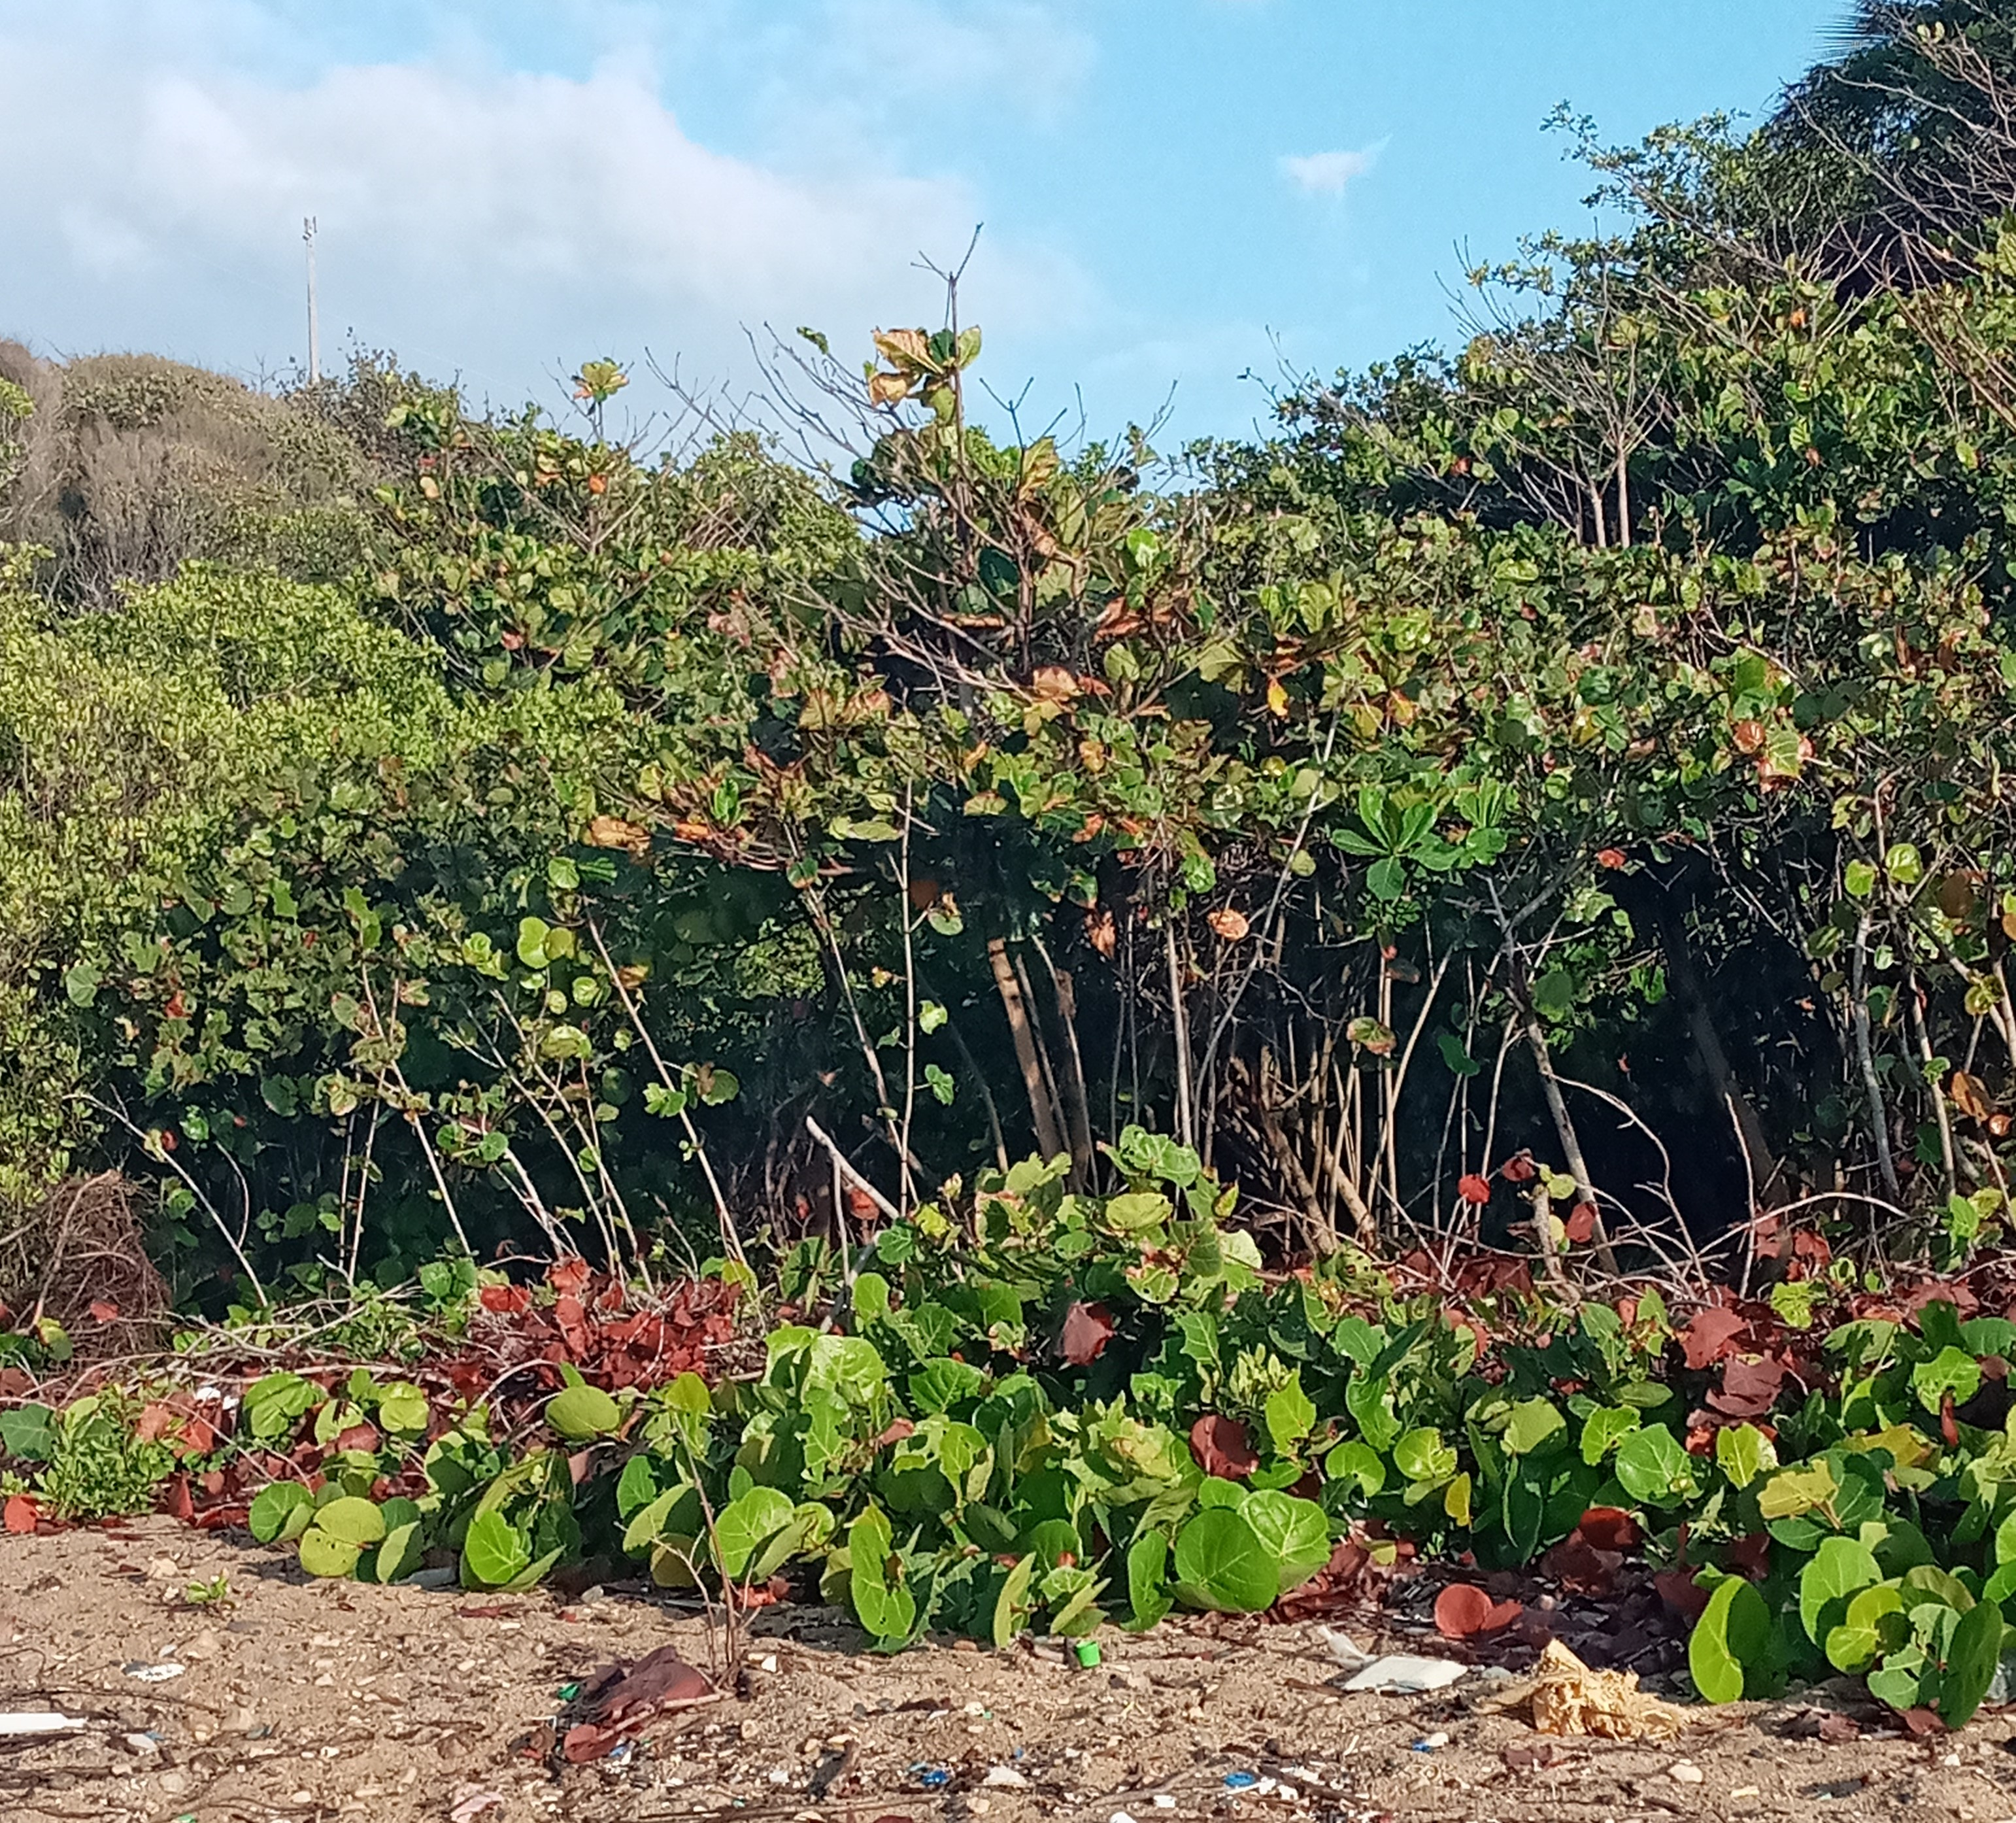
\includegraphics[height=3.12500in]{Cocoloba_uvifera.jpg}
\caption{Vegetación dunas de playa\label{cocoloba}}
\end{figure}

\begin{figure}
\centering
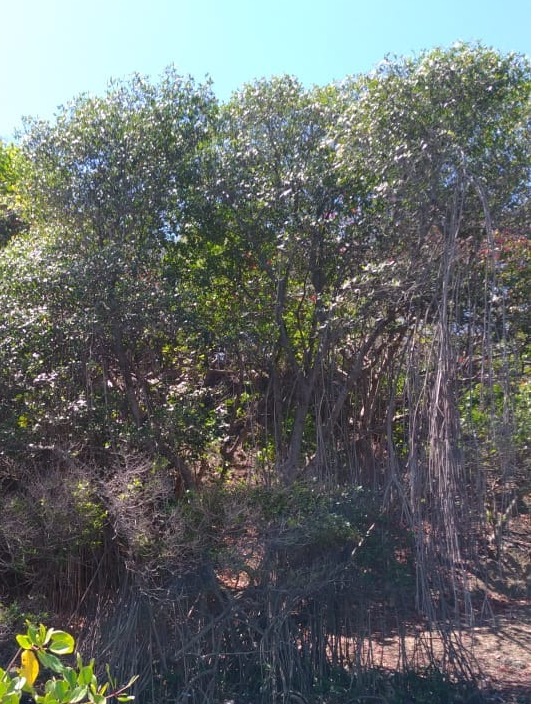
\includegraphics[height=3.38542in]{mangle_rojo.png}
\caption{Manglar\label{manglerojo}}
\end{figure}

\begin{figure}
\centering
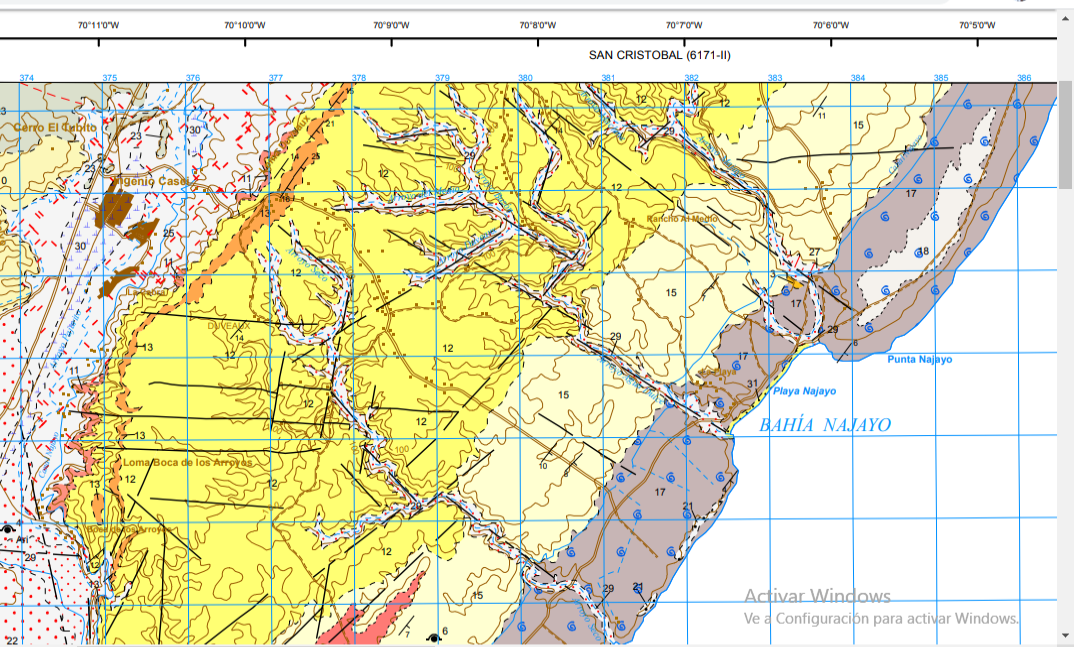
\includegraphics{mapa_bahia_najayo.png}
\caption{Mapa geológico escala 1:50,000 (hoja Nizao)\label{mapageo50k}}
\end{figure}

\ldots

\section{Metodología}\label{metodologuxeda}

Para cumplir los objetivos se emplearon varias técnicas, entre las que
se incluyen fotogrametría, navegación por satélite, teledetección,
sistemas de información geográfica y estadística.

Los cambios en el trazado de la línea de costa se analizaron utilizando
imágenes satelitales de Landsat 8 adquiridas entre los años 2013 y 2019.
De cada escena se extrajo la línea de costa empleando el algoritmo
CoastSat, el cual es un conjunto de herramientas escritas en Python, que
permite al usuario obtener series de tiempo de la posición de la costa
(Elsevier, n.d.).

Al delimitar las líneas de la costa, posteriormente se utilizó la
aplicación (QGIS y otros, n.d.) donde se seleccionaron los trazados de
mayor precisión teniendo como referencia la línea más antigua (2013),
dentro de dicho entorno gráfico se digitalizaron 25 transectos
perpendiculares a la dirección general del diseño. Finalmente, tanto los
transectos como las líneas fueron analizadas en R utilizando el script
RCoastSat (Batlle, 2020; R Core Team, 2020), el cual produjo resultados
gráficos que facilitaron la interpretación.

Asimismo, se colectaron muestras de sedimentos en siete puntos de
muestreos, los cuáles fueron seleccionados en base a dos áreas con
respecto al mar (berma y duna de playa) (ver figura \ref{muestras}).
Dichas muestras fueron depositadas en bolsas Whirl Pak de 23 cm L x 11.5
cm W, con 0.064 mm de grosor y 532 ml de capacidad. También, se tomaron
las coordenadas de cada punto con el receptor GPS convencional del
telefono personal y se midieron los clastos (en milímitros) presentes
con una regla en dos ejes (largo y ancho). Estos datos fueron rellenados
en un formulario electrónico para cada muestra, utilizando la aplicación
ODK Collection (Singh, 2013) descargada en el teléfono. Además, se
extrajo por medio de un martillo un fragmento del \emph{beachrock} (ver
figura \ref{clasto}) al cuál se le aplicó ácido clorhídrico para
determinar si contenía carbonato. Finalmente, para tener datos recientes
del perfil de la playa, se realizó un vuelo de dron y se tomaron
fotografias de la zona.

\ldots

\section{Resultados}\label{resultados}

\subsection{Cambio de líneas de
costa}\label{cambio-de-luxedneas-de-costa}

Los resultados generados se agrupan en tres subconjuntos: compilación de
trazados de la líneas de costa, colecta de sedimentos y las formaciones
de rocas en el centro de la playa, además de la restitución fotométrica
para la obtención de información tridimensional.

Los trazados en las líneas de costa permitieron reconstruir una serie
temporal que muestra la dinámica que envuelve el litoral a través del
tiempo. Los 25 transectos realizados sobre el límite costero
contribuyeron al mejoramiento de la obtención de datos (ver figura
\ref{transect_linea}). También estos mismos puntos muestran un esquema
del cambio de la costa por trimestre de cada año (ver figura
\ref{cambio_transecto}). Los cuales permitieron identificar los espacios
que son prospensos a presentar alteraciones en una época especifica (ver
tabla de resultos\ref{resultados}). Por consiguiente, el litoral exhibió
cambio en el tercer trimestre de los ocho periodo (septiembre-diciembre)
donde existió un proceso de agradación de la tierra hacia el mar casi
todos los años. En tanto que, los segundo trimestre (junio-agosto)
presentan una retrogradación del mar a la tierra.

\subsubsection{Rocas de playa}\label{rocas-de-playa}

La playa de Carlos pinto presenta rocas emergidas y submergidas en el
centro de la costa. Las mismas no exhiben elevadas altura, excepto las
que se encuentran cerca a los pequeños acantilados. Además, muestra tres
drenaje de agua continental que desembocan en el mar, en el mismo
espacio donde está distribuido el \emph{beachrock}.

\begin{figure}
\centering
\includegraphics{áreas_muestras_colectadas.jpg}
\caption{Áreas de muestras colectadas\label{muestras}}
\end{figure}

\begin{figure}
\centering
\includegraphics{Clasto_beachrock.jpg}
\caption{Composición de la roca de playa\label{clasto}}
\end{figure}

\begin{figure}
\centering
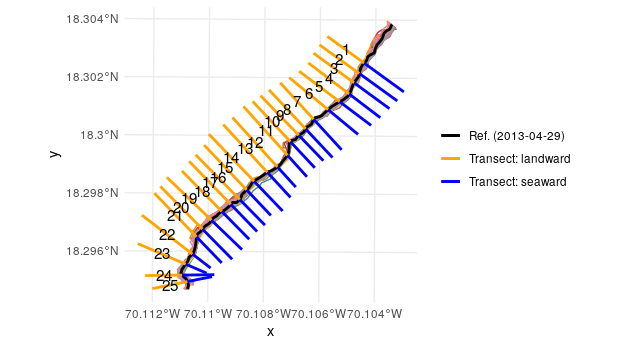
\includegraphics{transect_linea_R.png}
\caption{Transectos sobre las líneas costera de
playa\_Najayo\label{transect_linea}}
\end{figure}

La línea de color negro representa el trazado de referencia, el cual fue
extraído de la imágen satélital del año 2013. Los transectos de color
amarillo representan la superficie terrestre en tanto que los de azul el
mar.

\begin{figure}
\centering
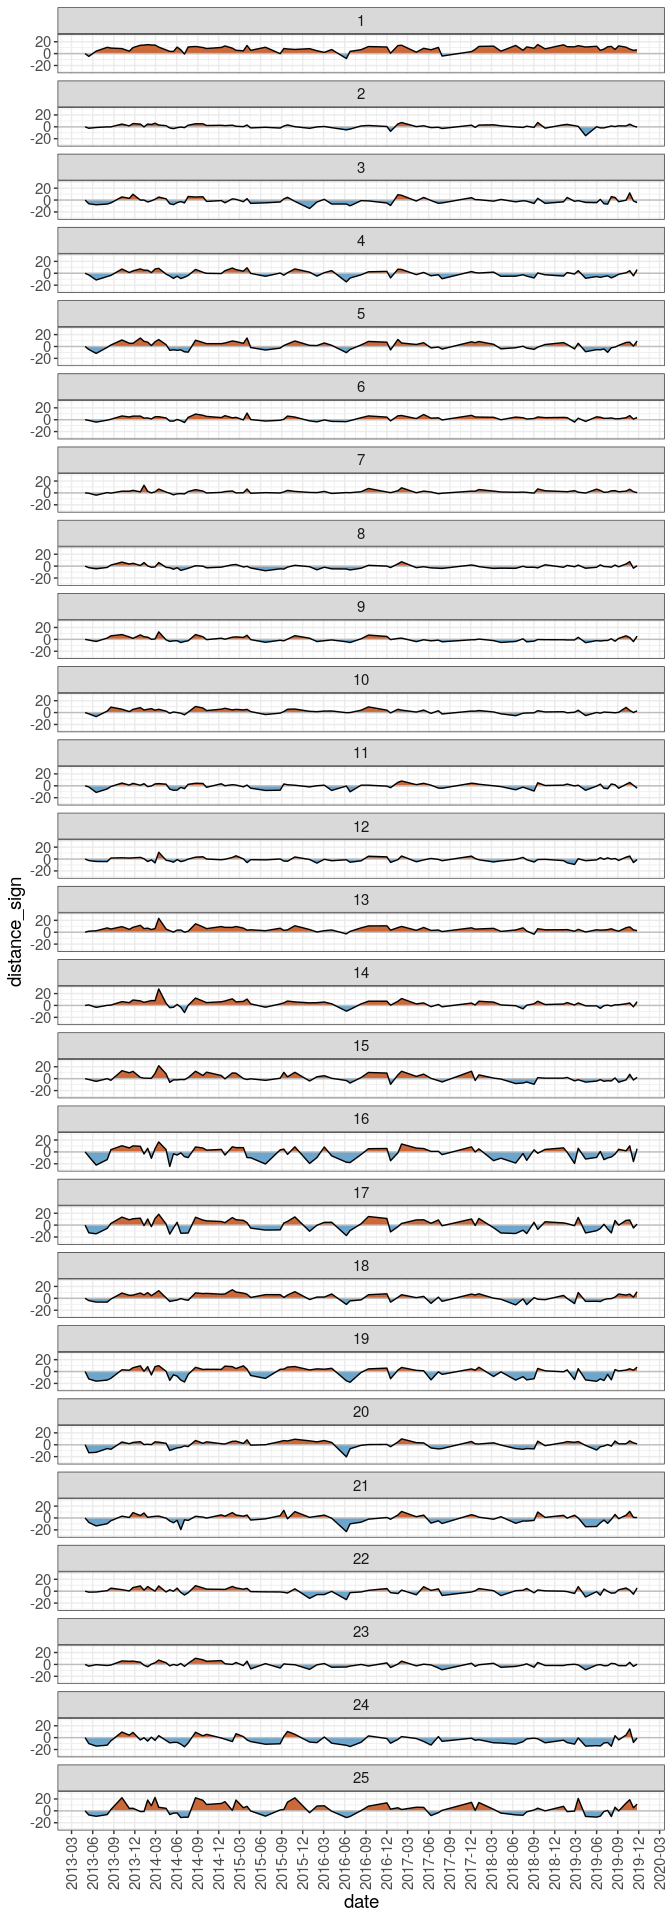
\includegraphics{cambio_playa_Najayo.png}
\caption{Transectos sobre las líneas costera de
playa\_Najayo\label{cambio_transecto}}
\end{figure}

\begin{figure}
\centering
\includegraphics{Beachrock.jpg}
\caption{Afloramiento de rocas playa\_Najayo\label{beachrock}}
\end{figure}

\begin{figure}
\centering
\includegraphics{Arroyo_Aguadulce.jpg}
\caption{Desembocadura arroyo Agua Dulce
Playa\_Carlos\_Pinto\label{arroyo_aguadulce}}
\end{figure}

\begin{figure}
\centering
\includegraphics{Resultados.png}
\caption{Tabla de resultados cambios enlíneas de
costa\label{resultados}}
\end{figure}

\ldots

\section{Discusión}\label{discusiuxf3n}

Los transectos sobre las diferentes líneas de costas muestran posibles
cambios del litoral en áreas espcíficas, el punto 25 representa una
variación dinámica en el trazado, en tanto que el punto uno no demuestra
alteración. Posiblemente estas variaciones sean producto en su monento
del incremento en el nivel del mar, a concecuencia de fenomenos
atmosféricos (tormentas/huracanes) ó por el deshielo de los polos por
causa del cambio climático. El mes de junio de todos los años presentó
cambios significativos en todos los trazados, donde el mar avanzó hacia
la tierra provablemente a concecuencia de el inicio de la temporada de
huracanes. Esto atribuyendo que el trimestre de junio-septiembre del
2016, fue el que más variedad mostró en cuanto al límite de costas,
llegando a superar los 20 m de distancia. Posiblemente esto se deba al
huracán Mathews de catégoria tres, el cual se encontra a unos 515 km
aproximadamente al suroeste de Santo Domingo.

\subsection{\texorpdfstring{\emph{Beachrock}}{Beachrock}}\label{beachrock}

Las rocas de la playa de Carlos Pinto (Najayo) por su ubicación en el
paso de una cañada que desemboca en el mar. Posiblemente se formó por la
compactación de la arena con el carbonato de calcio, es factible que en
este proceso de fosilización el agua continental circulara de manera
superficial por rocas calizas arrecifales. El \emph{beachrock} presenta
rocas alteradas de basaltos, fósiles y tonalidas las cuales
provablemente hallan emanado del continente y eventualmente llevadas
hasta ese lugar por la deriva continental, por la cañada que desemboca
en el mar o por un arroyo/río que tal vez hoy ya no transita en el
lugar.

\section{Agradecimientos}\label{agradecimientos}

\section{Información de soporte}\label{informaciuxf3n-de-soporte}

\ldots

\section{\texorpdfstring{\emph{Script}
reproducible}{Script reproducible}}\label{script-reproducible}

\ldots

\section*{Referencias}\label{referencias}
\addcontentsline{toc}{section}{Referencias}

\hypertarget{refs}{}
\hypertarget{ref-abad2007mapageonizao}{}
Abad de los Santos, M. (. (2007--2010). \emph{Mapa Geológico de la
República Dominicana a escala 1:50.000 de la hoja n 6170-I (Nizao) y
Memoria correspondiente}. Santo Domingo: Proyecto 1B de Cartografía
Geotemática de la República Dominicana. Programa SYSMIN. Servicio
Geológico Nacional.

\hypertarget{ref-abreu1999impacto}{}
Abreu, L. (1999). Impacto del turismo en el litoral de dominicana.
\emph{Revista Geográfica}, 167--182.

\hypertarget{ref-aliotta2009origen}{}
Aliotta, S., Spagnuolo, J. O., \& Farinati, E. A. (2009). Origen de una
roca de playa en la región costera de bahía blanca, argentina.
\emph{Pesquisas Em Geociências}, \emph{36}(1), 107--116.

\hypertarget{ref-rcoastsat}{}
Batlle, J. R. M. (2020). \emph{RCoastSat}.
\href{\%0Ahttps://github.com/geofis/RCoastSat\%0A}{
https://github.com/geofis/RCoastSat
}.

\hypertarget{ref-camara1997republica}{}
Cámara Artigas, R. (1997). \emph{República dominicana: Dinámica del
medio físico en la región caribe (geografía física, sabanas y litoral)
aportación al conocimiento de la tropicalidad insular}.

\hypertarget{ref-cervantes2009evidencia}{}
Cervantes Guerra, Y. M., Almaguer Carmenates, Y., Orozco Melgar, G.,
Pierra Conde, A., \& Gursky, H. (2009). \emph{Evidencia documental de
los cambios geomorfológicos en cayo moa grande, moa, cuba.}

\hypertarget{ref-codignotto1997geomorfologia}{}
Codignotto, J. (1997). \emph{Geomorfología y dinámica costera}.

\hypertarget{ref-maparecursosminerales}{}
Diaz de Neira, A. (2007--2010). \emph{Mapa de recursos minerales de la
Repú Dominicana, escala 1:100,000}. Santo Domingo: Proyecto 1B de
Cartografía Geotemática de la República Dominicana. Programa SYSMIN.
Servicio Geológico Nacional.

\hypertarget{ref-d1985manglares}{}
D'Croz, L. (1985). Manglares: Su importancia para la zona costera
tropical. \emph{Agonia de La Naturaleza}, 167--180.

\hypertarget{ref-vos2019coastsat}{}
Elsevier (Ed.). (n.d.). CoastSat: Un kit de herramientas python
habilitado para google earth engine para extraer costas de imágenes
satelitales disponibles públicamente. \emph{Environmental Modeling ~\&
Software}.

\hypertarget{ref-esquer2018modificacion}{}
Esquer, M. Z., Carreon, T. E., \& others. (2018). MODIFICACION de linea
de costa. \emph{Revista de Investigación Académica Sin Frontera:
División de Ciencias Económicas Y Sociales}, (16).

\hypertarget{ref-hernandez2008morfodinamica}{}
Hernández Santana, J. R., Ortiz Pérez, M. A., Méndez Linares, A. P., \&
Gama Campillo, L. (2008). Morfodinámica de la línea de costa del estado
de tabasco, méxico: Tendencias desde la segunda mitad del siglo xx hasta
el presente. \emph{Investigaciones Geográficas}, (65), 7--21.

\hypertarget{ref-kokot2004erosion}{}
Kokot, R. R. (2004). \emph{Erosión en la costa patagónica por cambio
climático}.

\hypertarget{ref-kokot2004vulnerabilidad}{}
Kokot, R. R., Codignotto, J. O., \& Elissondo, M. (2004).
\emph{Vulnerabilidad al ascenso del nivel del mar en la costa de la
provincia de río negro}.

\hypertarget{ref-polania1998manejo}{}
Polanía, J., \& Nat, R. (1998). Manejo de ecosistemas de manglar.
\emph{Memorias Del Curso Manejo de Ecosistemas de Manglar Y Arrecifes de
Coral. Bogotá}, 153--168.

\hypertarget{ref-qgis2015qgis}{}
QGIS y otros, E. de desarrollo de. (n.d.). QGIS sistema de información
geográfica. proyecto de fundación geoespacial de código abierto.
\emph{URL: Http: // Qgis. Osgeo Org}.

\hypertarget{ref-r2020r}{}
R Core Team. (2020). \emph{R: A language and environment for statistical
computing}. Retrieved from \href{\%0Ahttps://www.R-project.org/\%0A}{
https://www.R-project.org/
}

\hypertarget{ref-singh2013mobile}{}
Singh, H. (2013). Mobile data collection using an android device.
\emph{IJCST}, \emph{4}(1), 200--202.

\hypertarget{ref-suarez1999delimitacion}{}
Suárez de Vivero, J. L. (1999). Delimitación y definición del espacio
litoral. \emph{Jornadas Sobre El Litoral de Almería: Caracterización,
Ordenación Y Gestión de Un Espacio Geográfico Celebradas En Almería, 20
a 24 de Mayo de 1997. Pag: 13-23}.




\newpage
\singlespacing 
\end{document}
